% ===== UNIT 22: Matched-condition vs TransReID / CLIP-ReID (5.3) =====
% Status: REWRITTEN  (change to REWRITTEN / REVIEWED when done; see CHECKLIST.md)
% Rules: style rewrite only. Keep every \cite, \ref, \label, number, equation and table value as is. Change the wording, not the content.
\subsection{Matched-condition comparison with TransReID and CLIP-ReID}
\label{sec:matched}
The comparisons above apply post-processing to our pipeline, but they quote prior ViT-B baselines at their published operating points, which have no post-processing. We wanted to answer one central question: does our recipe or our post-processing produce the reported numbers? To answer it, we ran the official TransReID VeRi-776 checkpoint (\texttt{TransReID*} ViT-B/16, released by the TransReID authors~\cite{he2021transreid}) and the official CLIP-ReID ViT-B/16 VeRi-776 checkpoint~\cite{li2023clipreid} through our identical post-processing. This was AQE with $k{=}3$ and $k$-reciprocal re-ranking with $k_1{=}80,k_2{=}15,\lambda{=}0.2$. We used each repository's own released dataloader and inference path. Table~\ref{tab:matched} and Figure~\ref{fig:matched} show the results.

\begin{table}[!t]
  \centering
  \caption{Matched-condition comparison on VeRi-776: identical AQE $+$
    $k$-reciprocal re-ranking applied to each ViT-B/16 model's native inference
    feature. Both official baseline checkpoints, given our post-processing,
    exceed our own single stream. CLIP-ReID's base value is our re-extraction
    of its 512-D projection branch. Its published standalone figure is
    84.5\%~\cite{li2023clipreid}}
  \label{tab:matched}
  \small
  \begin{tabular}{L{5.0cm}C{1.8cm}C{2.0cm}C{2.4cm}}
    \toprule
    Model (native feature) & Feat.\ dim & Base mAP~(\%) & $+$\,our PP mAP~(\%) \\
    \midrule
    TransReID* (official)~\cite{he2021transreid} & 3840 & 82.11 & 91.12 \\
    CLIP-ReID (official)~\cite{li2023clipreid}   & 512  & 82.99 & \textbf{91.80} \\
    Ours (ViT-B/16 CLIP)                         & 1536 & 82.22 & 89.97 \\
    \bottomrule
  \end{tabular}
\end{table}

\begin{figure}[!t]
  \centering
  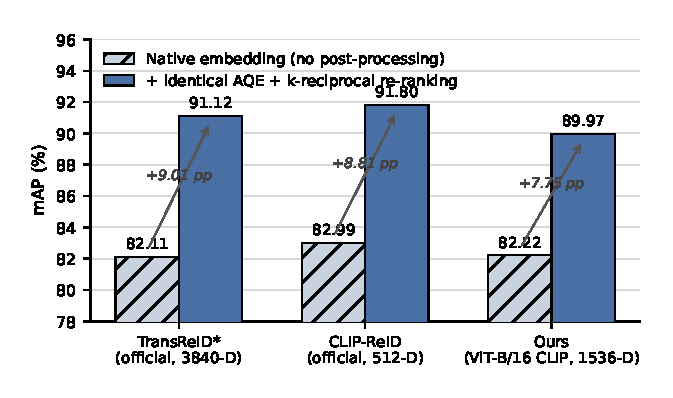
\includegraphics[width=0.92\columnwidth]{Fig4}
  \caption{Matched-condition comparison of three ViT-B/16 models on VeRi-776.
  Hatched bars are the native embeddings without post-processing. Solid bars
  add the identical AQE and $k$-reciprocal re-ranking. All three embeddings lie
  within 0.9\,pp of one another, and both official baselines re-rank to a
  higher final mAP than our own recipe}
  \label{fig:matched}
\end{figure}

The finding is clear. Once all three models get the same post-processing, the original TransReID reaches \textbf{91.12\%} mAP and the original CLIP-ReID \textbf{91.80\%}. Both are above our 89.97\%. At the raw-embedding level, all three are within 0.9\,pp of each other (82.11\,/\,82.99\,/\,82.22\%). The TransReID base value matches its published number ($\approx$82.3\%), so our extraction is faithful. The CLIP-ReID base value is 1.5\,pp below its published 84.5\%. We think this comes from the feature branch we chose in our re-extraction (the 512-D image projection from the authors' released inference path). This does not affect the matched comparison, because the same features give both the base and the post-processed numbers.

Our training recipe therefore gives no advantage over either baseline that is independent of post-processing. If anything, the native descriptors of both baselines re-rank slightly better than ours. This is not a perfectly matched feature-extraction comparison, because the three native descriptors differ in dimensionality and construction (3840-D global$+$JPM, 512-D CLIP projection, 1536-D concat-patch). But the conclusion holds despite this. The large ViT-B retrieval numbers reported here come from post-processing, not from changes to the recipe or the architecture. The same is probably true for much of the apparent progress after TransReID on this benchmark. So we present our single-stream result as a reproducible, specific baseline, not a superior recipe. The training-free fusion remains our main quantitative advance.
